\documentclass{article}

\input{C:/Users/ilden/Documents/School/TeX памятка/header.tex}

\begin{document}
	\tableofcontents
	\setcounter{tocdepth}{3}
	\newpage
	\section{Последовательности.}
	\begin{definition}
		Последовательность --- объекты (элементы), пронумерованные последовательными натуральными числами. Последовательности бывают как конечными, так и бесконечными.
	\end{definition}
	\begin{definition}
		Стационарная последовательность --- последовательность, у которой равны все элементы.
	\end{definition}
	\begin{note}
		Способы задания (правило, которое позволяет найти каждый элемент последовательности) последовательностей:
		\begin{itemize}
			\item Словесно/описательно.
			\item Таблица.
			\item Рекуррентно.
			\item Формульно.
		\end{itemize}
	\end{note}
	\subsection{Арифметическая прогрессия.}
	Пример: ряд натуральных чисел $1, 2, 3, \dots, n$.
	\begin{definition}
		Арифметическая прогрессия --- последовательность, где каждый следующий элемент увеличивается на фиксированную величину. $a_{n + 1} = a_n + d$, $d$ --- разность арифметической прогрессии.
	\end{definition}
	\begin{statement}
		Формулы.
		\begin{quote}
			$a_n = a_1 + (n - 1) \cdot d$. \\
			$a_n = \frac{a_{n + 1} + a_{n - 1}}{2} \rightarrow a_n = \frac{a_{n + k} + a_{n - k}}{2}$. \\
			$S_n = \frac{a_1 + a_n}{2} \cdot n = (a_1 + \frac{(n - 1) \cdot d}{2}) \cdot n = a_1 \cdot n + \frac{(n - 1) \cdot n}{2} \cdot d$.
		\end{quote}
	\end{statement}
	\subsection{Геометрическая прогрессия.}
	\begin{definition}
		Геометрической прогрессией называется такая последовательность, где первый член не нулевой, а каждый следующий в фиксированное число (не ноль) раз больше.
	\end{definition}
	\begin{definition}
		$b_n = b_{n - 1} \cdot q$, $q$ --- знаменатель ГП.
	\end{definition}
	\begin{definition}
		Если $|q| < 1$, тогда бесконечно убывающая ГП.
	\end{definition}
	\begin{statement}
		Формулы.
		\begin{quote}
			$S_n = \frac{b_{n + 1} - b_1}{q - 1} = \frac{b_1 \cdot (q^n - 1)}{q - 1}$. \\
			Для бесконечно убывающей ГП верно: $\frac{b_1}{b_2} = \frac{S}{S - b_1}$.
		\end{quote}
	\end{statement}
	\section{Производная и интеграл.}
	\begin{definition}
		Непрерывная функция~---
		\begin{enumerate}
			\item Можно нарисовать не отрывая руки.
			\item $\forall \varepsilon \exists \delta$.
			\item Совпадают левый и правый предел. (Если пойти слева и справа, то придем в одну точку.)
		\end{enumerate}
	\end{definition}
	\begin{statement}
		Производная точки касания~--- наклон касательной ($k = f'(x_0)$, $b = f(x_0) - f'(x_0) \cdot x_0$).
	\end{statement}
	\begin{statement}
		Полное уравнение касательной~--- $y = f'(x_0)(x - x_0) + f(x_0)$.
	\end{statement}
	\begin{definition}
		Уравнение нормали (перпендикуляра)~--- $y = -\frac{1}{f'(x_0)}(x - x_0) + f(x_0)$.
	\end{definition}
	\begin{property}
		\begin{enumerate}
			\item $f'(x) = \lim\limits_{\varDelta x \rightarrow 0} \frac{\varDelta y}{\varDelta x} = \lim\limits_{\varDelta x \rightarrow 0} \frac{f(x + \varDelta x) - f(x)}{\varDelta x}$.
			\item $f'(x) = 0$; $x_i$ - корни $=$ подозрительный экстремум.
			\item $f''(x) > 0 \Leftrightarrow$ выпукла вниз. $f''(x) < 0 \Leftrightarrow$ выпукла вверх.
			\item $(f^n(x))' = n \cdot f^{n - 1}(x) \cdot f'(x)$.
			\item $(f(x) + g(x))' = f'(x) + g'(x)$.
			\item $(f(x) \cdot g(x))' = f'(x) \cdot g(x) + f(x) \cdot g'(x)$.
			\item $(\frac{f(x)}{g(x)})' = \frac{f'(x) \cdot g(x) - f(x) \cdot g'(x)}{g^2(x)}$; $\Leftrightarrow f(x) \cdot g^{-1}(x)$.
			\item $(f(g(x)))' = f'(g(x)) \cdot g'(x)$.
		\end{enumerate}
	\end{property}
	\begin{property}
		\begin{enumerate}
			\item $(const)' = 0$.
			\item $(k \cdot x^n)' = kn \cdot x^{n - 1}$.
			\item $(k_1(k_2x + k_3)^n)' = nk_1(k_2x + k_3)^{n - 1} \cdot k_2$.
			\item $(\sin x)' = \cos x$.
			\item $(\cos x)' = - \sin x$.
			\item $tg'(x) = \frac{1}{cos^2(x)}$.
			\item $ctg'(x) = - \frac{1}{sin^2(x)}$.
			\item $(e^{f(x)})' = e^{f(x)} \cdot f'(x)$.
			\item $(a^x)' = a^x \cdot \ln a$.
			\item $(e^x)' = e^x$
			\item $(\ln x)' = \frac{1}{x}$
			\item $(\log_a x)' = \frac{1}{x \cdot \ln a}$
		\end{enumerate}
	\end{property}
	\section{Предел.}
	\begin{definition}[По Коши]
		$\lim \limits_{x \rightarrow x0} f(x) = A \Leftrightarrow \varepsilon > 0$ $\exists \delta: |x - x_0| < \delta$, то $|f(x) - A| < \varepsilon$ ($f(x_0) = A$).
	\end{definition}
	\begin{property}
		\begin{enumerate}
			\item $\lim \limits_{x \rightarrow x0} (f(x) \pm g(x)) = \lim \limits_{x \rightarrow x0} f(x) \pm \lim \limits_{x \rightarrow x0} g(x)$.
			\item $\lim \limits_{x \rightarrow x0} (f(x) \cdot g(x)) = \lim \limits_{x \rightarrow x0} f(x) \cdot \lim \limits_{x \rightarrow x0} g(x)$.
			\item $\lim \limits_{x \rightarrow a} f(x) = A$, $\lim \limits_{y \rightarrow A} = B$ $\Rightarrow$ $\lim \limits_{x \rightarrow a} g(f(x)) = B$.
			\item Правило Лапиталя. \\
			$\lim \limits_{x \rightarrow x0} f(x) = 0$, $\lim \limits_{x \rightarrow x0} g(x) = 0$ $\Rightarrow$ $\lim \limits_{x \rightarrow x0} \frac{f(x)}{g(x)} = \lim \limits_{x \rightarrow x0} \frac{f'(x)}{g'(x)}$.
		\end{enumerate}
	\end{property}
	\begin{statement}
		$\lim \limits_{x \rightarrow 0} \frac{sin(x)}{x} = 1$.
	\end{statement}
	\section{Показательная функция.}
	\begin{definition}
		$f(x) = a^x$, где $x$~--- независимая переменная, $a > 0$, $a \not= 1$.
	\end{definition}
	\begin{definition}
		Возведение в вещественную степень: $a^x = \lim\limits_{n \rightarrow \infty} a^{x_n}$, $x_n$~--- число $x$ с $n$ знаками после запятой $\Leftrightarrow x_n = \frac{\lfloor x \cdot 10^n \rfloor}{10^n}$.
	\end{definition}
	\begin{property}
		\begin{enumerate}
			\item $D(x) = \mathbb{R}$.
			\item $E(y) = (0; +\infty)$.
			\item $\uparrow \downarrow$
			\begin{itemize}
				\item $a \in (0; 1)$: $\downarrow$
				\item $a \in (1; \infty)$: $\uparrow$
			\end{itemize}
			\item Ограниченность. Снизу $0$.
			\item $\max/\min$. Нет.
			\item Асимптоты. $y = 0$.
			\item Монотонность. $\mathbb{R}$.
			\item Выпуклость. Выпукла вниз.
			\item График
			\begin{itemize}
				\item $a \in (0; 1)$
				\begin{figure}[H]
					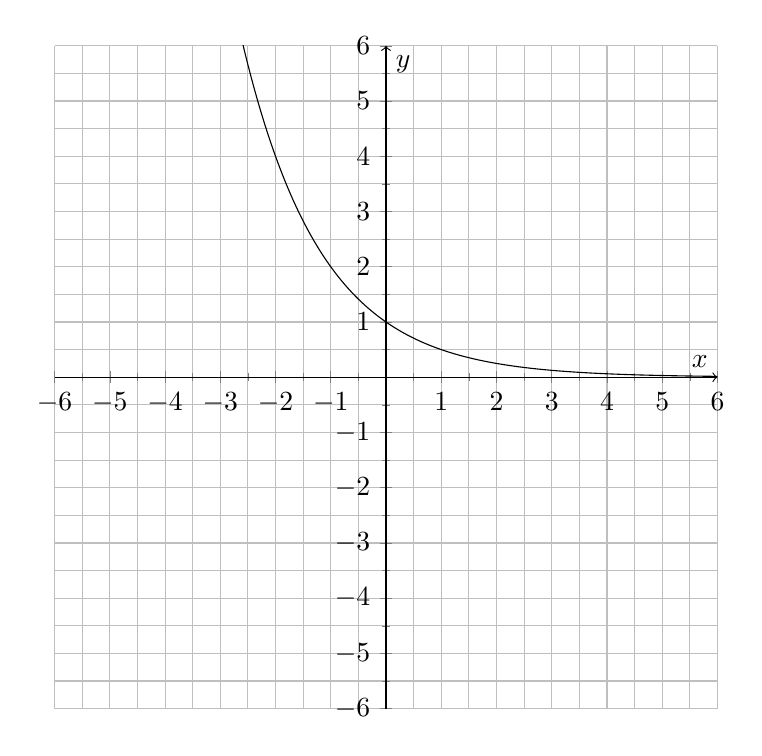
\begin{tikzpicture}
						\begin{axis}[
							width = 10cm, height = 10cm,
							grid = both,
							xmin = -6,
							xmax = 6,
							ymin = -6,
							ymax = 6,
							minor tick num = 1,
							axis equal,
							axis x line = middle,
							axis y line = middle,
							axis line style = {->, color=black},
							xtick distance = 1,
							ytick distance = 1,
							xlabel = {$x$},
							ylabel = {$y$},
							]
							\addplot[domain=-6:6, black, samples=200]{0.5^x};
						\end{axis}
					\end{tikzpicture}
				\end{figure}
				\item $a \in (1; \infty)$
				\begin{figure}[H]
					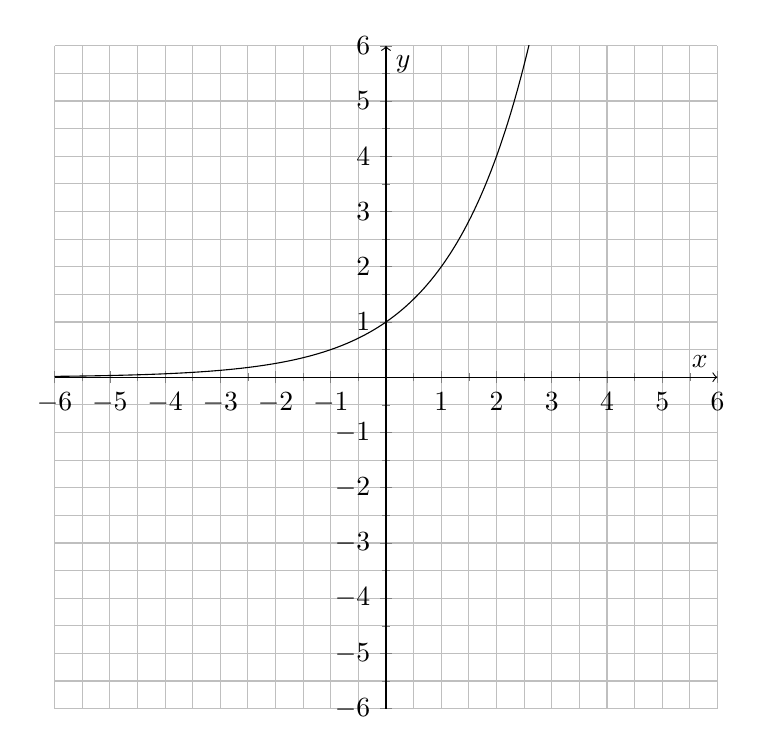
\begin{tikzpicture}
						\begin{axis}[
							width = 10cm, height = 10cm,
							grid = both,
							xmin = -6,
							xmax = 6,
							ymin = -6,
							ymax = 6,
							minor tick num = 1,
							axis equal,
							axis x line = middle,
							axis y line = middle,
							axis line style = {->, color=black},
							xtick distance = 1,
							ytick distance = 1,
							xlabel = {$x$},
							ylabel = {$y$},
							]
							\addplot[domain=-6:6, black, samples=200]{2^x};
						\end{axis}
					\end{tikzpicture}
				\end{figure}
			\end{itemize}
			\item Четность. Общего вида.
		\end{enumerate}
	\end{property}
	\section{Логарифм.}
	\begin{definition}
		$\log_ab$~--- логарифм числа $b$ по основанию $a$. $\log_ab$~--- такое число,что если возведем $a$ в эту степень, то получим $b$ ($a^{\log_ab} = b$); $a > 0, a\not=1, b > 0$.
	\end{definition}
	\begin{property}
		\begin{enumerate}
			\item $a^{\log_ab} = b$
			\item $\log_a(bc) = \log_a|b| + \log_a|c|$
			\item $\log_a(\frac{b}{c}) = \log_a|b| - \log_a|c|$
			\item $\log_ab^r = r\log_a|b|$
			\item $\log_{a^r}b = \frac{\log_{|a|}b}{r}$
			\item $\log_ab = \frac{\log_cb}{\log_ca}$
			\item $\log_ab = \frac{1}{\log_ba}$
			\item $\log_ab \cdot \log_ca = \log_cb$
			\item $a^{\log_bc} = c^{\log_ba}$
		\end{enumerate}
	\end{property}
	\begin{note}
		$\lg b = \log_{10}b$, $\ln b = \log_{e}b$.
	\end{note}
\end{document}
